\setcounter{chapter}{3}
\setcounter{rq}{1}


\chapter{Android Task Corpus}
\label{ch:android-corpus}



One of the challenges for characterizing task-relevant information as well as for proposing automatic techniques to automatically identify task-relevant text is
the lack of large corpora containing
software tasks and associated artifacts originating from heterogeneous sources.
To fill this gap, this chapter contributes with the Android tasks corpus (\textbf{\acs{DS-android}}), a dataset with 300 tasks comprising Android development and originating from Stack Overflow questions
as well as from GitHub issues on a variety of Android Open-Source Systems.



This chapter main contributions are \textit{(i)} the procedures for the corpus creation, and; \textit{(ii)} the corpus itself. A well-structured corpus lays the foundation for several studies that explore relationships between software tasks, natural language artifacts, and text within these artifacts. \red{eval \& corpus summary}





\section{Motivation}
\label{cp4:motivation}


When performing a software task, a software developer does not restrict her work
solely to coding~\cite{Meyer2017}.
Rather, there are many activities that a developer undertakes to complete a software task
as when they:



\begin{itemize}
    \item refer to API documentation or Q\&A websites for API usage purposes~\cite{umarji2008archetypal, Singer1998, robillard2011field};
    \item discuss in mailing lists a possible reusable library to be incorporated into their implementation~\cite{umarji2008archetypal, Bacchelli2012}; or
    \item confirm a system's behaviour referring to past discussions in community forums or in the system's documentation~\cite{Arya2019, Lotufo2012, Singer1998}.
\end{itemize}


A common aspect to these activities is the need to work with unstructured textual data, which comprises 80\% of the overall information created and used in enterprises~\cite{Bavota2014, holzinger2013}.
Due to such prevalence, there has been a large body of studies utilizing various techniques to extract
information from this text so that it can be embedded in
tools to software developers~\cite{Bavota2014, Xu2017, Robillard2015, Lotufo2012}. For instance, Xu et al. propose to mine relevant text from Stack Overflow
to generate answers to developers' technical question~\cite{Xu2017}
while FRAPT identifies key paragraphs explaining API elements in code tutorials~\cite{Jiang2017}.
As other examples, Lotufo et al. proposed a technique to identify sentences a developer would first read when inspecting bug reports~\cite{Lotufo2012} while Nadi and Treude investigated sentences that help a developer decide whether a Stack Overflow post is relevant to her task~\cite{nadi2020}.




Although these studies provide significant contributions, the fact that information to answer a question a developer has is usually located across many artifacts~\cite{Rastkar2013t} is often overlooked.
Hence existing techniques operate in an artifact-centric basis
what can be insufficient to provide to developers all the information needed
to completely and correctly accomplish a software task as several studies suggest that developers use heterogeneous sources to put together the information needed for task completion~\cite{josyula2018, Li2013, rao2020}.




We seek to design techniques that can scale to cover different types of artifacts
so that can be integrated into developers' information-seeking activities regardless of the artifact that a developer browses/inspects.
To design such techniques, we require a corpus with heterogeneous sources that a developer
might use to locate information relevant to her task.


\section{Methodology}
\label{cp4:methodology}

Corpus creation consists of three main steps, namely \textit{(1)} selection of tasks, \textit{(2)} selection of artifacts, and \textit{(3)} identification of relevant text within the selected artifacts. We detail each of these steps in the following sections.




\subsection{Software Tasks}
\label{cp4:corpus-tasks}


We consider a software task as a piece of work undertaken by a developer that often has to be finished within a certain time~\cite{2004merriam}.
Two common places a software task can be found are:

\begin{itemize}
    \item the description of a bug or feature request reported in a bug tracking systems; or in
    \item a post in a community forum, development mailing lists, and others.
\end{itemize}

GitHub issues or Stack Overflow (SO) posts are resources promptly available on the Web that align with our task definition.
In fact, several studies have used both as sources for software tasks~\cite{Arya2019, baltes2019, nadi2020, Xu2017}. Nonetheless, the sheer amount of data available on GitHub and Stack Overflow poses challenges to the selection of tasks for our corpus.
Baltes et al.~\cite{baltes2019} argues that even a cursory inspection of a sample set
of Stack Overflow posts shows clear differences in a post's content or structure due to aspects such as programming languages, frameworks, associated technologies, and others.


We scope task selection to
the \textit{Android} development domain as a means to define a common topic from which we can extract tasks from each source. This decision
restricts our selection to a single programming language (\textit{Java})
while it still allows us to investigate a domain that has been
widely discussed by practitioners and researchers alike.
For instance, over 35,000 developers have used Q\&A forums to discuss tasks covering 87\% of the Android API~\cite{parnin2012}
while researchers have investigated how changes to the Android SDK impact its ecosystem and development community~\cite{linares2014, bavota2014b, mcdonnell2013}.


\subsubsection{Stack Overflow tasks}

Provided that we restrict our corpus to tasks related to the Android development domain,
we randomly select 150 SO post from a curated list about Android development~\cite{baltes2019-rep}.


\textit{Saving WebView page to cache}~\cite{so18607655}
is the title of tasks in our corpus extracted from Stack Overflow. In this task, a developer describes the need
to
``\textit{save the website the first time it is connected to the internet so that a further connection is no longer needed}''.
To complete this task, a developer might refer to the Android Webview API~\cite{apiWebView}
or Q\&A forums about the Android cache system~\cite{so8410830}.


\subsubsection{GitHub tasks}

Since we are not aware of a comprehensive dataset of GitHub issues related to Android development, we devised our own strategy to fetch such data.


We selected 15 of top starred Android projects on GitHub by filtering the list of projects to the ones that contained the \textit{Java} and \textit{Android} tags.
For each of these projects, we randomly select 10 issues as the GitHub tasks of our corpus for a total of 150 distinct issues.
While selecting issues, we took care to check that they had at least one follow-up comment and that the issue title did not contain certain words, e.g., {\small \texttt{test}} or {\small  \texttt{ignore}},
so that our selection ignored issues automatically created by scripts or bots---a common pitfall that researchers must be aware of when mining GitHub~\cite{kalliamvakou2014}.




\textit{No lock screen controls ever}~\cite{git3578}
is an example of one of the issues in our corpus extracted from the \texttt{AntennaPod} open-source project.
Although the expected behaviour is that the app controls should be visible even with the screen locked,  a user reports that the app screen is missing.
A developer addressing this issue might review the Android lock task documentation~\cite{apiLockTask}
or refer to examples of applications that use the Android lock screen~\cite{mediumLockApp}.





\subsection{Artifact Selection}
\label{cp4:corpus-artifacts}


Our artifact selection approach seeks to simulate everyday practices on how developers search the Web~\cite{rao2020, Xia2017}. That is, we formulate a query for each task and use a Web search engine to retrieve artifacts that are pertinent to that task.


\subsubsection{Artifact sources}

As there are many different sources of artifacts, we restrict artifact selection to well known and studied sources~\cite{Starke2009,Kevic2014, Li2013}, i.e.,
Android and Java SE API documentation, Github issues, Stack Overflow answers; and Web tutorials or blog posts from Java and Android development.



\subsubsection{Query formulation}



We consider a task's title (i.e., SO question or GitHub issue title) as the seed used to search artifacts
using the \texttt{googlesearch} API~\cite{googlesearch}.
Coming up with proper search terms is a critical step of any search~\cite{Haiduc2013}
and, ideally, we should be able to formulate a query with terms able to retrieve exactly the most pertinent artifacts for a software task.
However, studies have shown that developers perform poorly in identifying good search terms~\cite{Starke2009,Kevic2014, Li2013} and thus, using a task's title
as an educated approximation to terms that a developer might use is a common procedure adopted by many studies in the field (e.g.,~\cite{Xu2017} or ~\cite{Silva2019}).







\subsubsection{Search results}


We fetch a maximum of 5 resources per artifact source --- a limitation necessary due to throttling or even blocking mechanisms in the APIs used to get the content of each source considered. We exclude search results that do not appear in the Amazon Alexa~\cite{alexa} Android Web pages traffic statistics in the period from April 2020 to March 2021. 
While applying this filter potentially decreased the number of artifacts per task, it ensured that results were indeed related to Android development. 
For instance, for a task discussing ``\textit{left and right swap}'' 
filtering avoided fetching unrelated resources, such as a Web page on  ``\textit{stock swap}''.
Table~\ref{tbl:googlesearch-example-git} shows one search result per artifact source for the GitHub task introduced in Section~\ref{cp4:corpus-tasks}.


Processing an artifact's content into a sequence of individual sentences 
followed procedures analogous to other studies in the field~\cite{Arya2019, nadi2020}.
Given a search result \texttt{URL}, we use \texttt{BeautifulSoup}~\cite{beautifulsoup4},
\texttt{StackAPI}~\cite{StackAPI} and \texttt{PyGithub}~\cite{PyGithub}
to fetch the artifacts' content and sentences in each paragraph
were identified using the Stanford CoreNLP toolkit~\cite{CoreNLP}.







\begin{table}[H]
\centering    
\begin{scriptsize}
\begin{threeparttable}
\rowcolors{2}{}{lightgray}    
\begin{tabular}{l|l}

\hline

\multicolumn{2}{c}{\textit{Saving WebView page to cache}}  \\

\hline
\hline

\multirow{1}{*}{API documentation}
& Managing WebView objects - Android Developers \\
% & WebView - Android Developers \\

\multirow{1}{*}{Github issues}
& WebView Caching contents WebView using the cachePolicy \\
% & Investigate whether removing WebView files on erase is a good idea \\


\multirow{1}{*}{StackOverflow answers}
& Android WebView not loading second page from cache \\
% & Save webview content for offline browsing? \\
\hline

\end{tabular}
\end{threeparttable}
\end{scriptsize}
\caption{Sample of artifacts obtained for a StackOverflow task~\cite{so18607655}}
\label{tbl:googlesearch-example-so}
\end{table}



\begin{table}[H]
\centering    
\begin{scriptsize}
\begin{threeparttable}
\rowcolors{2}{}{lightgray}    
\begin{tabular}{l|l}

\hline

\multicolumn{2}{c}{\textit{No lock screen controls ever}}  \\

\hline
\hline

\multirow{1}{*}{API documentation}
& Lock task mode - Android Developers \\
% & Recents Screen - Android Developers \\

\multirow{1}{*}{Github issues}
& Lock screen controls disappear on Android 11 \\
% & Bug: No lock screen image and controls \\


\multirow{1}{*}{StackOverflow answers}
& How to add MediaPlayer controls on lock screen? \\
% & How to disable home button in Android like lock screen apps do? \\



\multirow{1}{*}{Miscellaneous}
& Create A React Native App - Which works on Lock Screen (Android) \\

\hline


\end{tabular}
\end{threeparttable}
\end{scriptsize}
\caption{Sample of artifacts obtained for a Github task~\cite{git3578} }
\label{tbl:googlesearch-example-git}
\end{table}






\subsection{Relevant text detection}
\label{cp4:corpus-relevant-text}




 
We rely on state-of-the-art approaches able to automatically identify relevant text for the tasks and artifacts in our corpus~\cite{nadi2020, Robillard2015, Lotufo2012, Xu2017}.


We systematically reviewed related work and we identified techniques applicable to our domain problem. Selection criteria considered each technique's availability in existing replication packages and their readiness for use.
We also refrained from using approaches with training procedures (e.g., ~\cite{liu2020} or ~\cite{Treude2016}) because of the challenges related to parameter tuning~\cite{Chaparro2017, fucci2019}.



Based on these criteria, three techniques were selected for the following sources:


\begin{itemize}[leftmargin=\parindent, font=\normalfont\itshape]
    \item \texttt{\acs{AnsBot}} (\textit{SO Answers}) uses several features (e.g., information entropy, textual patterns, entity overlap, etc.) to determine that a sentence has useful information to a developer's technical question~\cite{Xu2017}.
    
    \item \texttt{\acs{Krec}} (\textit{API Documentation}) identifies text fragments that reflect ``potentially important text that programmers cannot afford to ignore when using the API''~\cite{Robillard2015}.
    
    \item \texttt{\acs{Hurried}} (\textit{GitHub issues}) identify the most relevant sentences in a bug report based on three factors used to assess a sentence's relevancy (i.e., sentence's prominence in the issue, topic, and its similarity to the task)~\cite{Lotufo2012}.
\end{itemize}


\art{Do I need to give details for miscellaneous?}

Tables~\ref{tbl:git-example-ansbot} to~\ref{tbl:git-example-hurried}
illustrate sentences selected by each approach\footnote{The number of sentences shown per technique
differs slightly due to a technique's input parameters and the length of the input artifact.}
 for pertinent artifacts retrieved for our Github lock screen task. 
% The techniques precision range from 71\% (\texttt{HurriedBug}) to 90\% (\texttt{APIRef}) and thus, we observe some unrelated sentences,
% such as a sentence expressing gratitude in Table~\ref{tbl:git-example-ansbot}.



\begin{table}[H]
\centering    
\begin{scriptsize}
\begin{threeparttable}
\rowcolors{2}{}{lightgray}
\begin{tabular}{ll}

\hline
\multicolumn{2}{c}{\textit{How to add MediaPlayer controls on lock screen?}} \\
\hline
\hline

1 & \parbox[l][.8cm][c]{10.5cm}{I had the same problem, and well, the solution was simple, do not use any widget, simply use the RemoteControlClientCompat class.} \\
2 & \parbox[l][.8cm][c]{10.5cm}{Here is my lockScreenControls() method code, which I call whenever I want to show this type of control (when plays a song).} \\
3 & \parbox[l][.5cm][c]{10.5cm}{Thank @ianhlake for the good 2 video} \\

\hline


\end{tabular}
\end{threeparttable}
\end{scriptsize}
\caption{Pertinent sentences automatically detected by \acs{AnsBot}}
\label{tbl:git-example-ansbot}
\end{table}

\begin{table}[H]
\centering    
\begin{scriptsize}
\begin{threeparttable}
\rowcolors{2}{}{lightgray}
\begin{tabular}{ll}
    
\hline
\multicolumn{2}{c}{\textit{Lock task mode - Android Developers}} \\
\hline
\hline

1 & \parbox[l][.8cm][c]{10.5cm}{You might use lock task mode if you're developing a kiosk application or a launcher to present a collection of apps.} \\
2 & \parbox[l][.8cm][c]{10.5cm}{To check if the current app is running in lock task mode, use the methods on ActivityManager as shown in the following example:} \\
3 & \parbox[l][.8cm][c]{10.5cm}{You can call KeyguardManager methods to find out if the device is locked and use an Activity lifecycle callback (such as onResume() that's called after unlocking) to start lock task mode.} \\
\hline

\end{tabular}
\end{threeparttable}
\end{scriptsize}
\caption{Pertinent sentences automatically detected by \acs{Krec}}
\label{tbl:git-example-krec}
\end{table}

\begin{table}[H]
\centering    
\begin{scriptsize}
\begin{threeparttable}
\rowcolors{2}{}{lightgray}
\begin{tabular}{ll}

\hline
\multicolumn{2}{c}{\textit{How to add MediaPlayer controls on lock screen?}} \\
\hline
\hline

1 & \parbox[l][.8cm][c]{10.5cm}{I had the same problem, and well, the solution was simple, do not use any widget, simply use the RemoteControlClientCompat class.} \\
2 & \parbox[l][.8cm][c]{10.5cm}{Here is my lockScreenControls() method code, which I call whenever I want to show this type of control (when plays a song).} \\
3 & \parbox[l][.5cm][c]{10.5cm}{Thank @ianhlake for the good 2 video} \\

\hline


\end{tabular}
\end{threeparttable}
\end{scriptsize}
\caption{Pertinent sentences automatically detected by \acs{Hurried}}
\label{tbl:git-example-hurried}
\end{table}





\subsection{Corpus Summary}
\textcolor{white}{force ident} % this is just for the chapter outline



Figure~\ref{fig:corpus-creation-pipeline} summarizes procedures for corpus creation.
We randomly sample a set of Android development tasks from Stack Overflow and GitHub
and use the Google search engine to find potential resources that might have
information for a task. We only consider resources highly ranked at Amazon Alexa and, for these resources, we apply state of the art techniques to detect relevant text in the artifact's content.



Overall, our corpus comprises 300 tasks evenly selected from SO and Git. 
There is a total of 262,278 sentences in 2,586 artifacts pertaining API documentation, Stack Overflow answers, Github issue discussions, and miscellaneous Web tutorials or blog posts. 



\begin{figure}
    \centering
    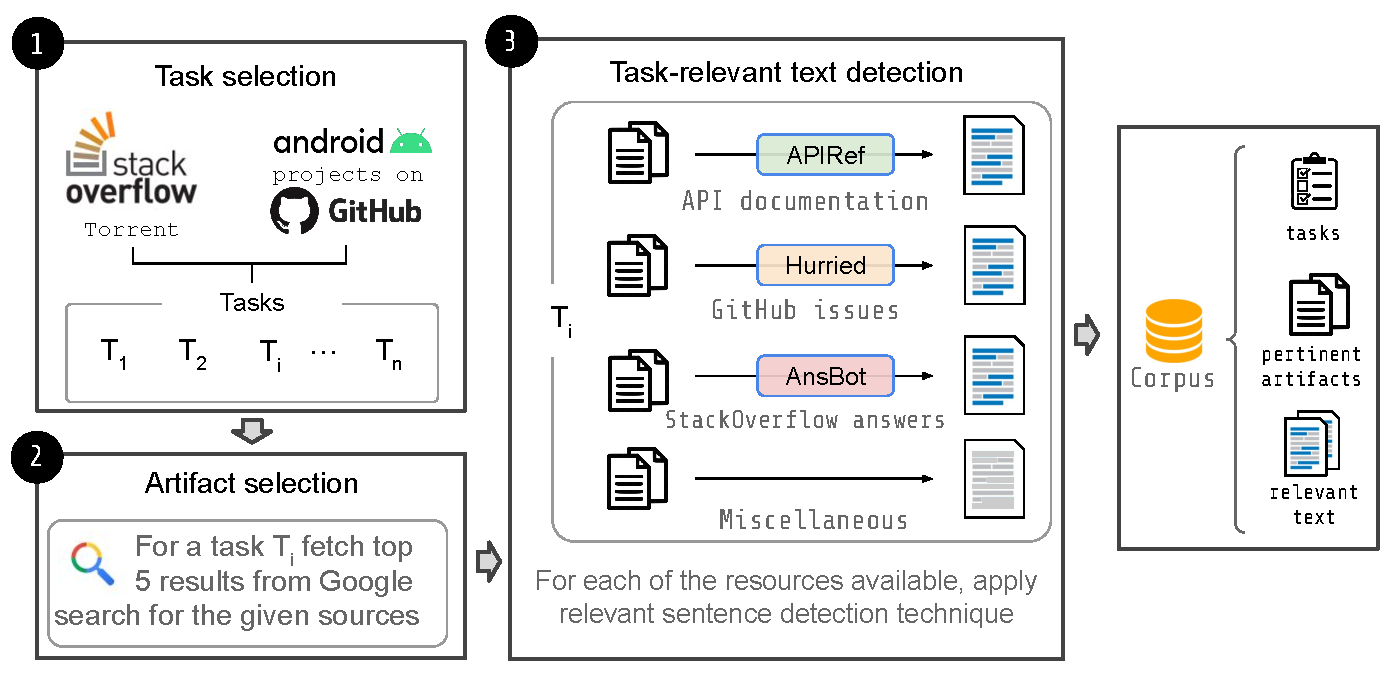
\includegraphics[width=\textwidth]{cp4/corpus-creation-pipeline}
    \caption{Summary of procedures for corpus creation}
    \label{fig:corpus-creation-pipeline}
\end{figure}




\clearpage

\section{Evaluation}
\label{cp4:evaluation}


To construct the \acs{DS-android} corpus, we apply a set of techniques 
to artifacts outside the ones where the techniques were originally proposed and evaluated.
For instance, \acs{AnsBot} was evaluated in a set of 100 general Java programming tasks~\cite{Xu2017} while our tasks comprise Android development.
Generalizability is a common threat emphasized in each of the techniques original studies~\cite{Xu2017, Lotufo2012, Robillard2015} and thus, there is a risk that the techniques do no apply to 
the tasks and artifacts in our corpus.




To mitigate this risk, we evaluate the accuracy of each technique on a subset of our corpus. We rely on three reference answers produced by 
experienced software developers to define \textit{golden relevant sentences} 
for a sample of 10 tasks and associated artifacts in our corpus. 
We use the golden data to evaluate and report each technique's accuracy in our corpus.
If we can show that the techniques identify relevant text with some \textit{margin of error},
future research can use our corpus for the design and comparison of techniques that identify task-relevant text automatically.


% --- To be able to judge that our techniques \textit{correctly} identify sentences relevant to a task,
% we require test data comprising sentences that contain information needed for task completion. \vspace{3mm}

% ---  this data for 10 tasks randomly sampled from the \acs{DS-android} corpus. \vspace{3mm}


% --- With this data, we report a technique's accuracy

% ------ For sources that have been evaluated in other studies, i.e., API documentation~\cite{Robillard2015}, GitHub issues~\cite{Lotufo2012}, and StackOverflow answers~\cite{Xu2017}, we compare the accuracy of our techniques 
% to the state-of-the-art

% ------ We also report our techniques accuracy on miscellaneous sources to show that our techniques apply to a variety of artifact sources



\subsection{Golden Data}


Creating golden data for the entirety of the \acs{DS-android} corpus is infeasible.
since it would require asking human evaluators to inspect thousands of artifacts and more than 260,000 sentences.
Due to this reason, we restrict this evaluation to a subset of 10 tasks evenly sampled from the two types of tasks in our corpus (i.e., 5 GitHub tasks and 5 Stack Overflow tasks). 
From now on, we refer to this subset as the \textbf{\acs{DS-android-small}} corpus.


For each one of the tasks in the \acs{DS-android-small} corpus, we also randomly selected 
one artifact per source type to a maximun of 4 artifacts per tasks, i.e., one API document, a Github issue discussion, one Stack Overflow answer, and a blog or Web tutorial.
Overall, this corpus has 2,375 sentences with an average of 64 sentences per artifact---
a size comparable to the \acs{DS-synthetic} corpus.
% ($\mypm$ 72)


We asked human evaluators to read the content of these artifacts and 
to mark sentences that they deemed useful and that provide information that assisted task completion.
Golden data in \acs{DS-android-small} consists of any sentence that two or more evaluators have deemed as useful for task-completion.



\subsubsection{Annotators}
\textcolor{white}{force ident} % this is just for the chapter outline

--- We recruited \red{n} graduate students with professional programming experience to produce \textit{golden} data for our tasks sample. \vspace{3mm}


\subsubsection{Annotation Procedures}
\textcolor{white}{force ident} % this is just for the chapter outline

Our intention is that goldens reflect text that a experienced developer would deem as useful for task completion and that they would share with someone eager to make their \textit{first contribution} in an open-source project.


To produce such data, annotators had  at their disposal a set of randomly assigned tasks description and links to artifacts pertinent to the respective task. We asked annotators to write a short plan (250 words max~\cite{Rastkar2010}) with instructions that a newcomer could follow to successfully complete the task. 
The purpose of the plan was to ensure that annotators built enough context about the task.
While perusing artifacts, annotators also had to manually highlight sentences that they deemed useful and that provide information that assisted task completion. 


The annotation process was facilitated by an in-house tool, in the form of a Web browser plugin shown in Figure~\ref{fig:corpus-annotation-tool}. In the figure, the top-right corner panel shows the browser extension. Annotators could start an annotation session and click the highlight buttom.
This would instrument the HTML of a page and identify each sentence in a paragraph. The tool allowd annotators to hove over individual sentences and select them as relevant by clicking on the hovered text (text in orange). For example, the figure depicts that an annotator deemed the sentence
``\textit{Call {\small \texttt{ActivityOptions.setLockTaskEnabled()}} ... when starting the activity}'' as relevant for the lock mode task.


\begin{figure}
    \centering
    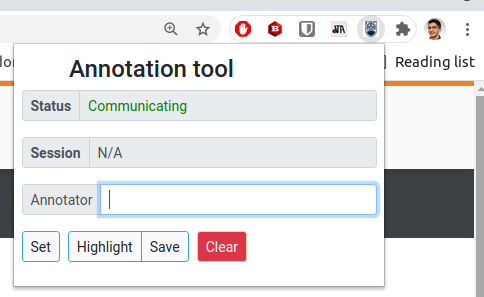
\includegraphics[width=\textwidth]{cp4/annotation-tool}
    \caption{Annotation tool and relevant sentences marked by an annotator}
    \label{fig:corpus-annotation-tool}
\end{figure}



\subsection{Method}
\textcolor{white}{force ident} % this is just for the chapter outline

% \gm{Separate the corpus creation from the method. Name each corpus.}

--- For each task, we have a set of artifacts with sentences identified by experienced developers that contain information relevant to the task \vspace{3mm}

--- We then apply the appropriate technique (baseline and ours) to automatically detect task-relevant text in that artifact

\gm{Where will the baseline techniques be explained? This is why I think you probably need to put corpus creation in a separate earlier chapter.}

--- We compute the technique's accuracy against the highlights in \acs{DS-android-small}

--- We use the obtained values to discuss the correctness of each technique






\subsubsection{Evaluation Metrics}
\textcolor{white}{force ident} % this is just for the chapter outline

--- We use the golden data in \acs{DS-android-small} to compute precision and recall


--- For a given task $t$ and artifact $a$, precision is computed as the ratio between the sentences identified that are indeed relevant (i.e., sentences highlighted by the annotators) and the total number of sentences identified by the technique


\begin{equation}
    Precision(t, a) = \frac{\# \text{\textit{sentences identified that were marked by annotators}}}{\# \text{\textit{sentences identified}}}
\end{equation}

\vspace{3mm}

--- Recall represents how many relevant sentences are identified by a technique


\begin{equation}
    Recall(t, a) = \frac{\# \text{\textit{sentences identified that were marked by annotators}}}{\text{\textit{total \# of sentences marked by annotators}}}
\end{equation}

\vspace{3mm}

--- When comparing techniques, we favor precision instead of recall because false positives may contribute to a developer abandoning reading of an artifact that would otherwise provide crucial information for her task~\cite{Rastkar2010}.


\subsection{Results}
\textcolor{white}{force ident} % this is just for the chapter outline

--- Discuss results \vspace{3mm}

\subsection{Threats to Validity}

--- Discuss threats \vspace{3mm}




% \acs{DS-android-small}

% \acs{DS-android-large}